\documentclass[11pt,a4paper]{article}

\usepackage[utf8]{inputenc}
\usepackage[T1]{fontenc}
% --- Español: usa babel-spanish si esta instalado (texlive-lang-spanish);
%     si no, define los rotulos a mano para que el documento compile igual.
\IfFileExists{spanish.ldf}{%
  \usepackage[spanish,es-noshorthands,es-tabla]{babel}%
}{%
  \PackageWarningNoLine{informe}{spanish.ldf no encontrado: se usan rotulos
    manuales y guionado ingles. Instalar texlive-lang-spanish para el guionado
    correcto}%
  \renewcommand{\abstractname}{Resumen}%
  \renewcommand{\contentsname}{\'Indice}%
  \renewcommand{\refname}{Referencias}%
  \providecommand{\bibname}{Referencias}\renewcommand{\bibname}{Referencias}%
  \renewcommand{\figurename}{Figura}%
  \renewcommand{\tablename}{Tabla}%
  \renewcommand{\listfigurename}{\'Indice de figuras}%
  \renewcommand{\listtablename}{\'Indice de tablas}%
  \renewcommand{\appendixname}{Ap\'endice}%
}
\usepackage{lmodern}
\usepackage{microtype}
\usepackage[margin=2.5cm]{geometry}
\usepackage{graphicx}
\usepackage{amsmath,amssymb}
\usepackage{booktabs}
\usepackage{longtable}
\usepackage{multirow}
\usepackage{float}
\usepackage{rotating}
\usepackage[font=small,labelfont=bf]{caption}
\usepackage{subcaption}
\usepackage{xcolor}
\usepackage{setspace}
\usepackage[numbers,sort&compress]{natbib}
\usepackage[colorlinks=true,linkcolor=black,citecolor=black,urlcolor=blue]{hyperref}

% --- rutas a las figuras generadas por los notebooks -----------------------
\graphicspath{{figuras/}}

% --- macros ----------------------------------------------------------------
\newcommand{\NDS}{\mathrm{NDS}}
\newcommand{\RS}{\mathrm{RS}}
\newcommand{\AUCcero}{\text{AUC}_{0.1}}
\newcommand{\fr}{f_{\mathrm{rank}}}
\newcommand{\rG}{r_{G}}
\newcommand{\rSS}{r_{SS}}
\newcommand{\rGe}{r_{G}^{\ast}}
\newcommand{\spn}[1]{\textit{#1}}
\newcommand{\unit}[2]{#1\,\mathrm{#2}}

\title{\bfseries Priorización de blancos terapéuticos y desorfanización de
compuestos bioactivos sobre un modelo de red multicapa quimiogenómica\\[2mm]
\large Reproducción y extensión del modelo de TDR~Targets sobre 16 especies}

\author{Gonzalo Giordano}
\date{7 de septiembre de 2026}

\begin{document}
\maketitle

\begin{abstract}
\noindent
El desarrollo de fármacos para enfermedades desatendidas está limitado por la
escasez de incentivos de mercado, lo que vuelve al reposicionamiento de drogas y
a la priorización computacional de blancos una estrategia central. Sobre la base
del modelo de red multicapa propuesto por Berenstein y colaboradores
\citep{berenstein2016} y de su implementación productiva en TDR~Targets
\citep{tdrtargets6}, en este trabajo se reconstruye el pipeline completo ---
caracterización de la red, barrido de parámetros del propagador, validación
cruzada y desorfanización de compuestos --- sobre una instantánea actualizada de
la base de datos, y se lo extiende con tres aportes propios: (i) una
caracterización cuantitativa de las capas y de su conectividad cruzada que
expone la asimetría de cobertura entre organismos modelo y patógenos;
(ii) un criterio de \emph{plateau} y de consistencia entre especies que muestra
que el óptimo del barrido no es un punto aislado sino una meseta amplia, con
$\beta = 1$ como único parámetro fuertemente seleccionado; y (iii) un criterio
operativo de decisión, $\rGe$, derivado de la curva de recuperación global de
pseudo-huérfanas, que define a partir de qué ranking una sugerencia deja de ser
distinguible del azar. La red integra $3{,}53 \times 10^{6}$ registros de
bioactividad compuesto--proteína sobre $3{,}99 \times 10^{5}$ proteínas de
30~especies. El barrido sobre 120~combinaciones de parámetros y 16~especies
alcanza $\AUCcero$ entre $0{,}58$ (\spn{M.~tuberculosis}) y $0{,}85$
(\spn{T.~cruzi}), reproduciendo los valores de la implementación de referencia.
Sobre \spn{P.~falciparum} el método reduce 233~compuestos fenotípicamente activos
a 12~casos tratables y produce dos sugerencias de blanco con $\rG = 15{,}5$, muy
por debajo del umbral $\rGe = 54$.
\end{abstract}

\tableofcontents
\clearpage

%============================================================================
\section{Introducción}
%============================================================================

Las enfermedades tropicales desatendidas afectan a alrededor de 1500~millones de
personas, mayoritariamente en países de ingresos bajos y medios, y han recibido
históricamente una inversión en investigación y desarrollo desproporcionadamente
baja respecto de su carga de enfermedad \citep{tdrtargets6}. En ese contexto, el
reposicionamiento de fármacos y la priorización computacional de blancos
proteicos son estrategias atractivas: permiten aprovechar información
experimental ya generada sobre organismos intensamente estudiados para guiar
decisiones sobre patógenos con muy poca caracterización propia.

El modelo de red multicapa de \citet{berenstein2016} formaliza esa idea. La red
tiene dos tipos de nodos --- compuestos y proteínas --- y tres clases de
enlaces: (a)~similitud química entre compuestos, (b)~asociaciones de
bioactividad compuesto--proteína medidas experimentalmente, y (c)~relaciones
funcionales entre proteínas, mediadas por su pertenencia a categorías de
ortología y de dominios proteicos. La priorización de blancos se plantea
entonces como un problema de propagación de un recurso (\emph{druggability})
desde un conjunto semilla de proteínas con inhibidores conocidos hacia el resto
del proteoma, a través de las categorías funcionales compartidas. El resultado
es un \emph{Network Druggability Score} (NDS) por proteína.

Este informe persigue tres objetivos:

\begin{enumerate}
  \item \textbf{Caracterizar} la instantánea actual de la base de datos: qué
    tamaño tiene cada capa, cómo se distribuye la información entre especies y
    qué artefactos introduce la capa de bioactividad
    (Sección~\ref{sec:red}).
  \item \textbf{Reproducir y auditar} el procedimiento de priorización: barrer
    el espacio de parámetros del propagador, medirlo con validación cruzada
    interna, verificar que los óptimos coinciden con la implementación de
    referencia, y caracterizar la \emph{forma} del óptimo, no sólo su ubicación
    (Sección~\ref{sec:priorizacion}).
  \item \textbf{Aplicar} el modelo al problema inverso --- dado un compuesto
    activo sin blanco conocido, sugerir proteínas candidatas --- calibrando el
    procedimiento con un experimento de pseudo-huérfanas y derivando un umbral
    de decisión explícito, que luego se usa sobre compuestos antipalúdicos
    huérfanos reales (Secciones~\ref{sec:huerfanas} y~\ref{sec:pfal}).
\end{enumerate}

Respecto del trabajo original, los aportes propios de esta realización son la
caracterización cuantitativa de la conectividad cruzada entre especies
(Sección~\ref{sec:conectividad}), el diagnóstico y la corrección del sesgo por
compuestos promiscuos de bajo peso molecular (Sección~\ref{sec:promiscuidad}),
el análisis de \emph{plateau} y consistencia del barrido
(Sección~\ref{sec:plateau}) y la definición del umbral $\rGe$
(Sección~\ref{sec:umbral}).

%============================================================================
\section{Materiales y métodos}
%============================================================================

\subsection{Datos}

Todos los resultados provienen de una única instantánea de la base de datos,
cuyas tablas y fechas de corte se registran automáticamente en los archivos
\texttt{*\_meta.json} de cada corrida. Las tablas centrales son las
bioactividades compuesto--proteína (corte 7~de agosto de 2026), las
bioactividades compuesto--organismo (4~de junio de 2026), las afiliaciones
InterPro \citep{interpro} (10~de junio de 2026) y OrthoMCL \citep{orthomcl}
(25~de agosto de 2026), y los \emph{clusterings} químicos por
\emph{fingerprint} \citep{rogers2010} y por subestructura (13~de mayo de 2026).
El análisis se ejecutó con Python~3.12.2 y pandas~2.2.3.

El estudio se restringe a 16~especies que combinan organismos modelo
intensamente caracterizados (\spn{H.~sapiens}, \spn{M.~musculus},
\spn{S.~cerevisiae}, \spn{E.~coli}, \spn{A.~thaliana}, \spn{D.~melanogaster},
\spn{C.~elegans}, \spn{O.~sativa}, \spn{D.~discoideum}) y patógenos de interés
sanitario (\spn{M.~tuberculosis}, \spn{S.~aureus}, \spn{P.~falciparum},
\spn{T.~brucei}, \spn{T.~cruzi}, \spn{L.~major}, \spn{C.~albicans}).

\subsection{El propagador y sus cuatro parámetros}
\label{sec:metodo}

Sea $A = (a_{i\ell})$ la matriz de afiliación proteína--categoría, con
$k_i = \sum_\ell a_{i\ell}$ el número de categorías de la proteína~$i$ y
$|\ell| = \sum_i a_{i\ell}$ el tamaño de la categoría~$\ell$. Sea $w_j$ el peso
semilla de la proteína~$j$ (no nulo sólo para proteínas con inhibidores
conocidos). El puntaje se calcula en dos pasos: primero cada categoría acumula
recurso de sus proteínas semilla,
%
\begin{equation}
  f_\ell \;=\; \underbrace{|\ell|^{-\beta}}_{\text{corrección de tamaño}}
               \cdot \underbrace{\RS_\ell(\alpha)}_{\text{relevancia}}
               \cdot \sum_{j} a_{j\ell}\,\frac{w_j}{k_j^{\lambda_j}},
  \label{eq:fl}
\end{equation}
%
y luego cada proteína recoge el recurso de sus categorías,
%
\begin{equation}
  \NDS_i \;=\; k_i^{\,\lambda_i - 1}\sum_\ell a_{i\ell}\, f_\ell .
  \label{eq:nds}
\end{equation}
%
Los cuatro parámetros libres tienen lecturas distintas:

\begin{description}
  \item[$\alpha$ (relevancia).] $\RS_\ell$ se obtiene de un test exacto de
    Fisher que evalúa el enriquecimiento de proteínas semilla dentro de la
    categoría~$\ell$; $\alpha$ reescala esos $p$-valores (corregidos por FDR
    \citep{benjamini1995}) para convertirlos en un peso. Con $\alpha = 0$ todas
    las categorías pesan igual.
  \item[$\beta$ (tamaño de categoría).] Penaliza a las categorías muy pobladas,
    que de otro modo dominan la propagación por puro volumen. El caso
    $\beta = 0$ corresponde a la red $G'_r$ del trabajo original y $\beta > 0$ a
    $G'_{rk}$.
  \item[$\lambda$ (difusión).] Controla cuánto se diluye el recurso de una
    proteína entre sus categorías. Además de los valores fijos
    $\lambda \in \{0;\,0{,}5;\,1\}$ se admite un modo \emph{híbrido} en el que
    $\lambda$ se calcula por proteína como
    $\lambda_i = (k_i / k_{\max})^{\gamma}$.
  \item[$\gamma$ (exponente del híbrido).] Sólo interviene cuando $\lambda$ es
    híbrido; con $\lambda$ fijo el modelo lo ignora. Por eso la grilla efectiva
    tiene 120~combinaciones y no~240.
\end{description}

La grilla barrida fue
$\alpha \in \{0;\,0{,}3;\,0{,}6;\,0{,}9;\,1{,}2\}$,
$\beta \in \{0;\,0{,}5;\,1;\,1{,}5\}$,
$\lambda \in \{0;\,0{,}5;\,1;\,\text{híbrido}\}$ y
$\gamma \in \{0{,}8;\,1{,}0;\,1{,}2\}$.

\subsection{Métrica de evaluación}

Para cada especie y cada combinación de parámetros se evalúa la capacidad del
NDS de recuperar las proteínas \emph{druggables} conocidas de esa especie. Dado
que en la práctica sólo interesa el extremo superior del ranking, la métrica no
es el área bajo la curva ROC completa sino el área parcial restringida a
$\text{FPR} \le 0{,}10$, normalizada y corregida por el método de
\citet{mcclish1989} para que el azar valga $0{,}5$ y el clasificador perfecto
valga~$1$. Notamos esta métrica $\AUCcero$. Se reporta además la AUC global como
referencia.

\subsection{Reproducibilidad}

Cada notebook escribe sus tablas, figuras y un \texttt{meta.json} con los
parámetros, las versiones de las librerías y las fechas de corte de cada tabla
consumida. Los resultados de esta corrida se validaron contra la
implementación de referencia (\texttt{genoma\_completo\_v5}) exigiendo
coincidencia exacta del vector $(\alpha,\beta,\lambda,\gamma)$ óptimo en las
16~especies.

%============================================================================
\section{Resultados}
%============================================================================

\subsection{Dimensiones y cobertura de la red}
\label{sec:red}

La Tabla~\ref{tab:dimensiones} resume el tamaño de cada capa. La red integra
$3{,}53 \times 10^{6}$ registros de bioactividad compuesto--proteína, de los
cuales $248\,545$ constituyen enlaces positivos y $144\,552$ negativos; el
resto queda como indeterminado. La capa de afiliaciones aporta $769\,661$
enlaces proteína--categoría sobre $14\,083$ categorías InterPro y $76\,157$
categorías OrthoMCL.

\begin{table}[H]
\centering
\caption{Dimensiones de las capas del modelo en la instantánea analizada.}
\label{tab:dimensiones}
\small
\begin{tabular}{llr}
\toprule
Capa & Entidad & $n$ \\
\midrule
1 --- compuestos      & compuestos con bioactividad          & $949\,054$ \\
2 --- proteínas       & proteínas ($V_P$)                    & $399\,352$ \\
2 --- proteínas       & especies                             & $30$ \\
3 --- afiliaciones    & categorías InterPro                  & $14\,083$ \\
3 --- afiliaciones    & categorías OrthoMCL                  & $76\,157$ \\
2--3 (afiliación)     & enlaces proteína--categoría          & $769\,661$ \\
1--2 (bioactividad)   & registros compuesto--proteína        & $3\,526\,999$ \\
1--2 (bioactividad)   & enlaces $E_{DP}$ positivos           & $248\,545$ \\
1--2 (bioactividad)   & enlaces $E_{DP}$ negativos           & $144\,552$ \\
1--2 (bioactividad)   & proteínas \emph{druggables}          & $19\,650$ \\
fenotípica            & registros compuesto--organismo       & $931\,971$ \\
\bottomrule
\end{tabular}
\end{table}

La distribución de esa información entre especies es fuertemente desigual
(Figura~\ref{fig:disponibilidad}). \spn{H.~sapiens} concentra 1985~proteínas
\emph{druggables} sobre 18\,052 proteínas anotadas, mientras que patógenos como
\spn{T.~cruzi} y \spn{L.~major} tienen 29 y 30 respectivamente sobre proteomas de
$19\,245$ y $6564$ proteínas. Es exactamente el desbalance que justifica el
enfoque: sin transferencia de información entre organismos, los patógenos no
tienen suficiente evidencia propia para sostener una priorización.

La cobertura de anotaciones muestra un patrón complementario. La afiliación
OrthoMCL es casi universal en eucariotas (\spn{P.~falciparum} y \spn{L.~major}
alcanzan el $100\,\%$; \spn{A.~thaliana}, el $99{,}8\,\%$), mientras que la
cobertura InterPro es sistemáticamente menor y cae justamente en los protozoos:
$44{,}7\,\%$ en \spn{P.~falciparum}, $40{,}3\,\%$ en \spn{T.~brucei} y
$39{,}6\,\%$ en \spn{T.~cruzi}, frente a $65{,}4\,\%$ en \spn{H.~sapiens} y
$71{,}5\,\%$ en \spn{M.~musculus}. La consecuencia práctica es que en los
patógenos de interés la propagación descansa más sobre ortología que sobre
dominios.

\begin{figure}[H]
\centering

\includegraphics[width=\textwidth]{01_f01_disponibilidad}
\caption{Disponibilidad de información por especie: tamaño del proteoma,
cobertura de anotaciones InterPro y OrthoMCL, y número de proteínas
\emph{druggables}. El contraste entre organismos modelo y patógenos motiva la
transferencia de información en red.}
\label{fig:disponibilidad}
\end{figure}

Las categorías funcionales tienen una distribución de grado marcadamente
sesgada (Figura~\ref{fig:grado}). Unas pocas categorías InterPro genéricas
--- dominio quinasa (IPR000719, 9576~proteínas), sitios de unión a ATP
(IPR017452, 3772) o dedos de zinc (IPR013087, 3605) --- concentran una fracción
desproporcionada de los enlaces, mientras que la enorme mayoría de las
categorías conecta a un puñado de proteínas. Esta cola pesada es precisamente lo
que el parámetro $\beta$ de la Ecuación~\eqref{eq:fl} está diseñado para
compensar.

\begin{figure}[H]
\centering
\begin{subfigure}{0.49\textwidth}
  
\includegraphics[width=\textwidth]{01_f02_grado_afiliaciones}
  \caption{Distribución de grado.}
\end{subfigure}\hfill
\begin{subfigure}{0.49\textwidth}
  
\includegraphics[width=\textwidth]{01_f03_tramos_de_grado}
  \caption{Enlaces acumulados por tramo de grado.}
\end{subfigure}
\caption{Grado de las categorías de afiliación (InterPro y OrthoMCL). Un número
reducido de categorías muy pobladas acumula una fracción sustancial de los
enlaces proteína--categoría.}
\label{fig:grado}
\end{figure}

\subsection{Estructura de la capa química}

Los \emph{clusterings} químicos por \emph{fingerprint} y por subestructura
producen distribuciones de tamaño de \emph{cluster} igualmente sesgadas
(Figura~\ref{fig:clusters}a): el \emph{cluster} mayor por \emph{fingerprint}
agrupa 510~compuestos, pero la moda está en tamaño~1. El grafo de similitud
química está además muy fragmentado (Figura~\ref{fig:clusters}b): sobre
$192\,742$ componentes conexas, la componente gigante contiene $137\,050$
\emph{clusters}, de los cuales sólo $2818$ tienen alguna bioactividad asociada.
Es decir, la mayor parte del espacio químico está poblada por compuestos sin
información experimental de blanco: el problema de las moléculas huérfanas no es
marginal sino la situación por defecto.

\begin{figure}[H]
\centering
\begin{subfigure}{0.49\textwidth}
  
\includegraphics[width=\textwidth]{02_f01_tamanos_cluster}
  \caption{Tamaños de \emph{cluster}.}
\end{subfigure}\hfill
\begin{subfigure}{0.49\textwidth}
  
\includegraphics[width=\textwidth]{02_f02_componentes_conexas}
  \caption{Componentes conexas.}
\end{subfigure}
\caption{Estructura de la capa química. La fragmentación del grafo de similitud
y la escasez de bioactividad anotada en la componente gigante delimitan el
alcance de la inferencia química.}
\label{fig:clusters}
\end{figure}

\subsection{Conectividad cruzada entre especies}
\label{sec:conectividad}

Para cuantificar cuánta información puede efectivamente transferirse entre
organismos se calcularon dos matrices de conectividad: el número de categorías
de afiliación compartidas entre cada par de especies
(Figura~\ref{fig:conectividad}a) y el número de compuestos con bioactividad
positiva compartidos (Figura~\ref{fig:conectividad}b).

Las dos matrices cuentan historias distintas. La conectividad por anotaciones es
alta y bien estructurada por filogenia: \spn{H.~sapiens} y \spn{M.~musculus}
comparten $13\,740$ categorías, los tripanosomátidos entre sí comparten entre
$5669$ y $7287$, y \spn{P.~falciparum} mantiene entre $2400$ y $3200$ categorías
compartidas con casi todos los eucariotas del panel. Incluso los pares
filogenéticamente distantes conservan cientos o miles de categorías en común.

La conectividad química, en cambio, es órdenes de magnitud más pobre y está
dominada por un único nodo. \spn{H.~sapiens} comparte 648~compuestos con
\spn{P.~falciparum}, 512 con \spn{M.~musculus} y 819 con \spn{S.~cerevisiae}; pero
\spn{P.~falciparum} comparte apenas 16~compuestos con \spn{L.~major} y 12 con
\spn{T.~cruzi}. Fuera de la fila y la columna humanas, la matriz es
prácticamente vacía.

Esta asimetría es, a nuestro juicio, el hallazgo estructural más relevante de la
caracterización: el puente que sostiene la transferencia de información entre
patógenos no es la evidencia química directa --- que casi no existe entre
pares de patógenos --- sino la capa de afiliaciones funcionales. Justifica
\emph{a posteriori} que el propagador de las Ecuaciones~\eqref{eq:fl}
y~\eqref{eq:nds} opere sobre categorías y no sobre similitud química.

\begin{figure}[H]
\centering
\begin{subfigure}{0.49\textwidth}
  
\includegraphics[width=\textwidth]{02_f03_conectividad_anotaciones}
  \caption{Categorías compartidas.}
\end{subfigure}\hfill
\begin{subfigure}{0.49\textwidth}
  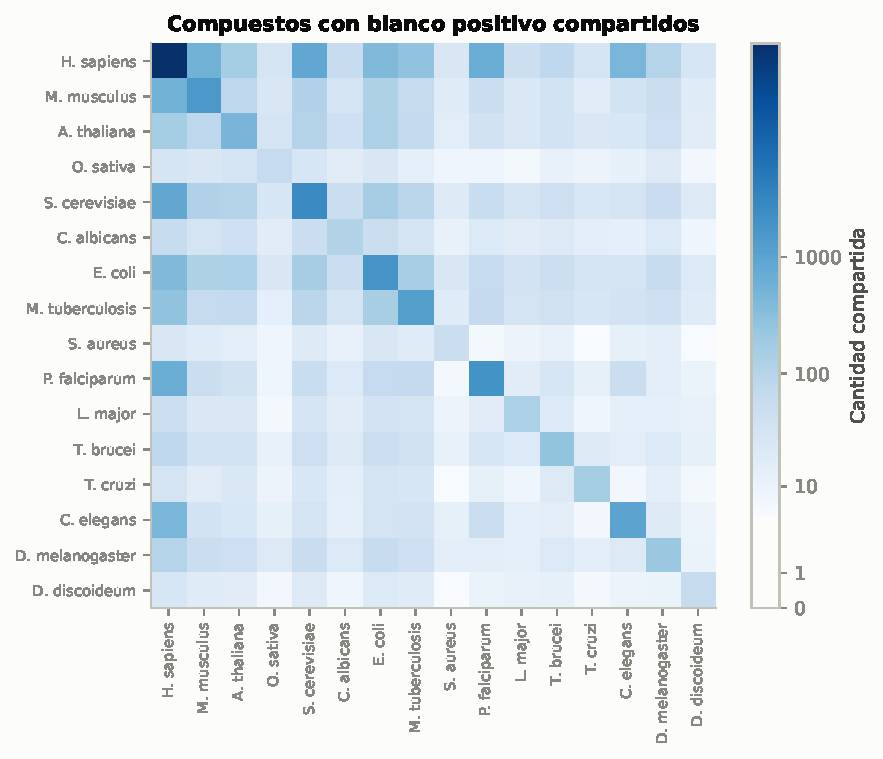
\includegraphics[width=\textwidth]{02_f04_conectividad_drogas}
  \caption{Compuestos compartidos.}
\end{subfigure}
\caption{Conectividad cruzada entre las 16~especies. La capa de afiliaciones
funcionales (a)~conecta densamente a todos los organismos, mientras que la
evidencia química compartida (b)~es escasa y está concentrada en
\spn{H.~sapiens}.}
\label{fig:conectividad}
\end{figure}

\subsection{Calidad de la capa de bioactividad y compuestos promiscuos}
\label{sec:promiscuidad}

La clasificación de los $3{,}53 \times 10^{6}$ registros compuesto--proteína
arroja $88{,}7\,\%$ de registros indeterminados, $7{,}0\,\%$ positivos y
$4{,}1\,\%$ negativos, con sólo un $0{,}17\,\%$ de registros inconsistentes
(Figura~\ref{fig:tags}). La baja tasa de inconsistencia indica que el criterio
de consolidación de bioactividades es estable.

\begin{figure}[H]
\centering

\includegraphics[width=0.72\textwidth]{03_f01_bioactividades_por_tag}
\caption{Clasificación de los registros de bioactividad compuesto--proteína.
La abrumadora mayoría queda como indeterminada; los inconsistentes son
marginales.}
\label{fig:tags}
\end{figure}

Un problema más serio aparece al examinar la promiscuidad. Un puñado de
compuestos está asociado a decenas de miles de proteínas parentales: el más
extremo (\texttt{drug\_id}~166536, $\mathrm{MW} = 114{,}1$) aparece vinculado a
$30\,584$ proteínas; le siguen 1116907 ($\mathrm{MW} = 128{,}2$, $24\,544$
proteínas) y 163058 ($\mathrm{MW} = 142{,}2$, $21\,196$ proteínas). Todos ellos
son moléculas muy pequeñas: no se trata de inhibidores promiscuos genuinos sino,
casi con certeza, de fragmentos, buffers y artefactos de anotación.

Estos compuestos son tóxicos para el modelo porque actúan como atajos que
conectan proteínas sin ninguna relación funcional real. Se definió por lo tanto
un filtro conjunto sobre peso molecular y promiscuidad,
$\mathrm{MW} < 150$ y $N_{\text{parentales}} > 100$, cuyo efecto se muestra en
la Tabla~\ref{tab:filtro}: elimina apenas 30~compuestos ($0{,}015\,\%$ del
total) pero remueve $104\,075$ aristas, el $11{,}98\,\%$ de la capa de
bioactividad. La relación entre ambas cifras --- tres órdenes de magnitud ---
es la que justifica el filtro: es una intervención mínima con un efecto
estructural grande. La Figura~\ref{fig:promiscuidad} muestra que la elección de
los umbrales no es crítica, ya que la curva de aristas filtrables se estabiliza
en un rango amplio.

\begin{table}[H]
\centering
\caption{Impacto del filtro de compuestos promiscuos de bajo peso molecular.}
\label{tab:filtro}
\small
\begin{tabular}{lrrrr}
\toprule
Criterio & Compuestos & \% compuestos & Aristas & \% aristas \\
\midrule
$\mathrm{MW} < 150$ y $N_{\text{par.}} > 100$ & $30$ & $0{,}015$ & $104\,075$ & $11{,}98$ \\
\bottomrule
\end{tabular}
\end{table}

\begin{figure}[H]
\centering

\includegraphics[width=\textwidth]{03_f02_promiscuidad}
\caption{Promiscuidad por compuesto en función del peso molecular y curva de
sensibilidad del filtro. Los compuestos hiperconectados se agrupan en la región
de bajo peso molecular, compatible con fragmentos y artefactos de anotación más
que con farmacología real.}
\label{fig:promiscuidad}
\end{figure}

Este filtro se aplica aguas arriba de todo el análisis de desorfanización de la
Sección~\ref{sec:huerfanas}.

%----------------------------------------------------------------------------
\subsection{Priorización de blancos: barrido de parámetros}
\label{sec:priorizacion}

Con la red caracterizada y filtrada, se barrieron las 120~combinaciones válidas
de $(\alpha,\beta,\lambda,\gamma)$ sobre cada una de las 16~especies, evaluando
en cada caso la recuperación de las proteínas \emph{druggables} conocidas.
La Figura~\ref{fig:positivos} muestra el conjunto de positivos disponible por
especie, que fija el techo estadístico de cada evaluación.

\begin{figure}[H]
\centering

\includegraphics[width=0.8\textwidth]{01_f01_positivos_por_especie}
\caption{Número de proteínas \emph{druggables} (positivos) por especie. Las
especies con pocos positivos producen estimaciones de $\AUCcero$ con mayor
varianza.}
\label{fig:positivos}
\end{figure}

\paragraph{Control frente a la implementación de referencia.}
Antes de interpretar los resultados se verificó que la reimplementación
reproduce la corrida de referencia \texttt{genoma\_completo\_v5}: el vector de
parámetros óptimo coincide en las 16~especies y las diferencias de $\AUCcero$
son numéricamente despreciables (Figura~\ref{fig:control}). El pipeline queda
así validado como reproducción fiel antes de introducir cualquier extensión.

\begin{figure}[H]
\centering

\includegraphics[width=0.8\textwidth]{01_f02_control_v5}
\caption{Control de reproducibilidad contra la implementación de referencia.
Coincidencia de los parámetros óptimos en las 16~especies.}
\label{fig:control}
\end{figure}

\paragraph{Desempeño por especie.}
La Tabla~\ref{tab:optimos} y la Figura~\ref{fig:auc01} resumen el resultado. El
$\AUCcero$ óptimo varía entre $0{,}581$ (\spn{M.~tuberculosis}) y $0{,}849$
(\spn{T.~cruzi}). El ordenamiento es informativo: los mejores desempeños
corresponden a \spn{T.~cruzi} ($0{,}849$), \spn{T.~brucei} ($0{,}789$),
\spn{L.~major} ($0{,}743$) y \spn{P.~falciparum} ($0{,}736$) --- es decir, a los
protozoos patógenos, que son justamente el objetivo del método --- mientras que
los peores corresponden a \spn{M.~tuberculosis} ($0{,}581$), \spn{S.~cerevisiae}
($0{,}581$), \spn{S.~aureus} ($0{,}591$) y \spn{H.~sapiens} ($0{,}594$).

La lectura no es que el método funcione mejor en protozoos por alguna virtud
biológica, sino que allí la señal disponible es más aprovechable: en especies
con muchos positivos y con \emph{druggables} distribuidos por todo el proteoma
--- el caso humano --- la propagación desde semillas ya no agrega tanto sobre lo
que se sabe. La AUC global, en cambio, es alta y relativamente uniforme
(entre $0{,}743$ y $0{,}883$), lo que confirma que la métrica restringida al
extremo del ranking es la que discrimina realmente entre configuraciones.

\begin{table}[H]
\centering
\caption{Parámetros óptimos y desempeño por especie. $N$: proteínas evaluadas;
$\lambda = \text{híb.}$ indica modo híbrido, en el que rige $\gamma$.}
\label{tab:optimos}
\small
\begin{tabular}{llrrrrrr}
\toprule
Especie & $(\alpha,\beta,\lambda,\gamma)$ & $\AUCcero$ & AUC & Youden & $N$ \\
\midrule
\spn{T.~cruzi}          & $(0{,}0;\,1{,}0;\,1{,}0;\,0{,}8)$      & $0{,}849$ & $0{,}883$ & $0{,}721$ & $19\,241$ \\
\spn{T.~brucei}         & $(0{,}3;\,1{,}5;\,\text{híb.};\,0{,}8)$ & $0{,}789$ & $0{,}844$ & $0{,}642$ & $8633$ \\
\spn{L.~major}          & $(0{,}0;\,1{,}5;\,0{,}5;\,0{,}8)$      & $0{,}743$ & $0{,}859$ & $0{,}679$ & $6564$ \\
\spn{P.~falciparum}     & $(1{,}2;\,1{,}0;\,1{,}0;\,0{,}8)$      & $0{,}736$ & $0{,}841$ & $0{,}624$ & $5495$ \\
\spn{A.~thaliana}       & $(0{,}0;\,1{,}0;\,0{,}5;\,0{,}8)$      & $0{,}683$ & $0{,}828$ & $0{,}567$ & $21\,714$ \\
\spn{C.~elegans}        & $(0{,}3;\,1{,}5;\,1{,}0;\,0{,}8)$      & $0{,}664$ & $0{,}781$ & $0{,}553$ & $27\,425$ \\
\spn{D.~discoideum}     & $(0{,}0;\,1{,}0;\,1{,}0;\,0{,}8)$      & $0{,}652$ & $0{,}871$ & $0{,}759$ & $13\,088$ \\
\spn{C.~albicans}       & $(1{,}2;\,1{,}0;\,0{,}5;\,0{,}8)$      & $0{,}645$ & $0{,}868$ & $0{,}661$ & $6040$ \\
\spn{O.~sativa}         & $(1{,}2;\,1{,}0;\,0{,}5;\,0{,}8)$      & $0{,}644$ & $0{,}843$ & $0{,}580$ & $22\,012$ \\
\spn{D.~melanogaster}   & $(0{,}0;\,1{,}0;\,1{,}0;\,0{,}8)$      & $0{,}614$ & $0{,}812$ & $0{,}570$ & $10\,695$ \\
\spn{M.~musculus}       & $(0{,}3;\,1{,}0;\,\text{híb.};\,0{,}8)$ & $0{,}611$ & $0{,}818$ & $0{,}538$ & $18\,185$ \\
\spn{H.~sapiens}        & $(0{,}0;\,0{,}5;\,1{,}0;\,0{,}8)$      & $0{,}594$ & $0{,}769$ & $0{,}481$ & $16\,301$ \\
\spn{S.~aureus}         & $(0{,}3;\,0{,}5;\,0{,}5;\,0{,}8)$      & $0{,}591$ & $0{,}878$ & $0{,}715$ & $2187$ \\
\spn{E.~coli}           & $(1{,}2;\,1{,}0;\,1{,}0;\,0{,}8)$      & $0{,}588$ & $0{,}820$ & $0{,}565$ & $4533$ \\
\spn{S.~cerevisiae}     & $(0{,}9;\,0{,}0;\,0{,}0;\,0{,}8)$      & $0{,}581$ & $0{,}743$ & $0{,}445$ & $6093$ \\
\spn{M.~tuberculosis}   & $(1{,}2;\,1{,}0;\,\text{híb.};\,0{,}8)$ & $0{,}581$ & $0{,}866$ & $0{,}656$ & $4073$ \\
\bottomrule
\end{tabular}
\end{table}

\begin{figure}[H]
\centering

\includegraphics[width=0.85\textwidth]{01_f03_auc01_por_especie}
\caption{$\AUCcero$ óptima por especie. Los protozoos patógenos, objetivo
primario del método, ocupan las primeras posiciones.}
\label{fig:auc01}
\end{figure}

La Figura~\ref{fig:roc} detalla el caso de \spn{P.~falciparum}: la curva ROC
completa y la distribución de NDS bajo la configuración óptima
$(\alpha,\beta,\lambda,\gamma) = (1{,}2;\,1{,}0;\,1{,}0;\,0{,}8)$. La separación
entre proteínas \emph{druggables} y el resto se concentra en la cola derecha de
la distribución de puntajes, que es exactamente la región que $\AUCcero$ mide.

\begin{figure}[H]
\centering
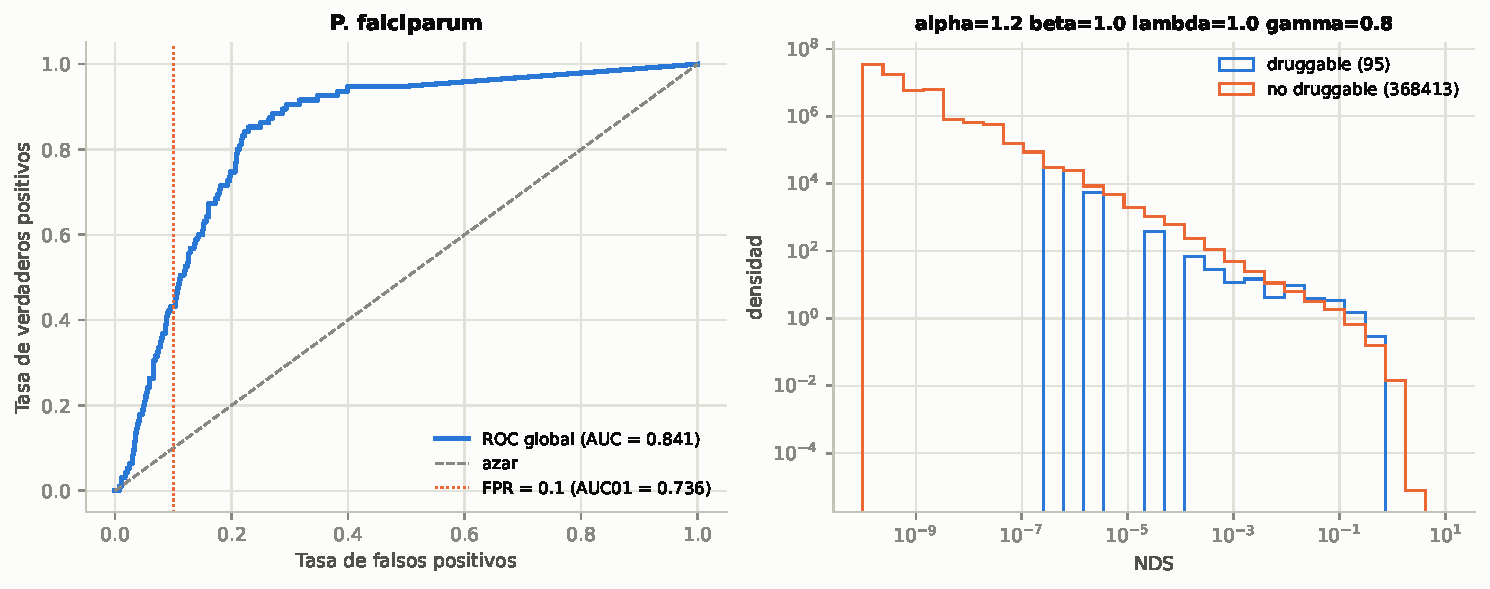
\includegraphics[width=\textwidth]{02_f01_roc_pfal}
\caption{\spn{P.~falciparum} bajo su configuración óptima: curva ROC global
(izquierda) y distribución de NDS discriminada por condición de
\emph{druggable} (derecha).}
\label{fig:roc}
\end{figure}

\subsection{Forma del óptimo: \emph{plateau} y consistencia}
\label{sec:plateau}

Reportar un único vector óptimo por especie invita a una lectura equivocada, la
de que el método requiere una calibración fina y específica. Para evaluar eso se
analizó la \emph{forma} del óptimo, no sólo su ubicación.

\paragraph{El óptimo es una meseta.}
La Tabla~\ref{tab:plateau} muestra la caída relativa de $\AUCcero$ al pasar del
mejor vector al quinto, décimo y vigésimo mejor, junto con el número de
combinaciones que quedan dentro de tolerancias absolutas de $0{,}001$, $0{,}005$
y $0{,}01$. La caída al quinto mejor no supera el $1{,}2\,\%$ en ninguna especie
y es inferior al $0{,}3\,\%$ en la mitad de ellas. En \spn{S.~cerevisiae},
48~de las 120~combinaciones caen dentro de $0{,}01$ del máximo; en
\spn{M.~musculus}, 44; en \spn{A.~thaliana}, 35. El óptimo no es un pico agudo
sino una meseta amplia (Figura~\ref{fig:plateau}), lo que implica que el
desempeño del método es robusto frente a errores de calibración.

\begin{table}[H]
\centering
\caption{Caracterización del \emph{plateau}. Caída relativa de $\AUCcero$
respecto del máximo y número de combinaciones (sobre 120) dentro de cada
tolerancia absoluta.}
\label{tab:plateau}
\small
\begin{tabular}{lrrrrrrr}
\toprule
\multirow{2}{*}{Especie} & \multirow{2}{*}{$\AUCcero^{\max}$}
 & \multicolumn{3}{c}{caída (\%) al $k$-ésimo} & \multicolumn{3}{c}{$n$ dentro de} \\
\cmidrule(lr){3-5}\cmidrule(lr){6-8}
 & & $k{=}5$ & $k{=}10$ & $k{=}20$ & $0{,}001$ & $0{,}005$ & $0{,}01$ \\
\midrule
\spn{T.~cruzi}        & $0{,}849$ & $0{,}43$ & $0{,}82$ & $1{,}09$ & 2 & 5  & 16 \\
\spn{T.~brucei}       & $0{,}789$ & $0{,}24$ & $0{,}48$ & $1{,}14$ & 3 & 10 & 13 \\
\spn{L.~major}        & $0{,}743$ & $0{,}23$ & $0{,}30$ & $1{,}55$ & 2 & 12 & 17 \\
\spn{P.~falciparum}   & $0{,}736$ & $0{,}65$ & $1{,}40$ & $1{,}90$ & 2 & 4  & 8  \\
\spn{A.~thaliana}     & $0{,}683$ & $0{,}21$ & $0{,}52$ & $0{,}83$ & 1 & 8  & 35 \\
\spn{C.~elegans}      & $0{,}664$ & $0{,}80$ & $1{,}12$ & $1{,}54$ & 1 & 3  & 7  \\
\spn{D.~discoideum}   & $0{,}652$ & $1{,}12$ & $1{,}59$ & $2{,}14$ & 2 & 2  & 4  \\
\spn{C.~albicans}     & $0{,}645$ & $0{,}14$ & $0{,}29$ & $1{,}36$ & 2 & 13 & 18 \\
\spn{O.~sativa}       & $0{,}644$ & $0{,}18$ & $0{,}24$ & $0{,}46$ & 1 & 21 & 29 \\
\spn{D.~melanogaster} & $0{,}614$ & $0{,}82$ & $1{,}08$ & $1{,}56$ & 1 & 3  & 7  \\
\spn{M.~musculus}     & $0{,}611$ & $0{,}10$ & $0{,}16$ & $0{,}34$ & 4 & 24 & 44 \\
\spn{H.~sapiens}      & $0{,}594$ & $1{,}05$ & $1{,}82$ & $2{,}14$ & 1 & 2  & 4  \\
\spn{S.~aureus}       & $0{,}591$ & $0{,}17$ & $0{,}79$ & $1{,}60$ & 3 & 8  & 11 \\
\spn{E.~coli}         & $0{,}588$ & $0{,}31$ & $0{,}47$ & $0{,}78$ & 2 & 10 & 20 \\
\spn{S.~cerevisiae}   & $0{,}581$ & $0{,}06$ & $0{,}10$ & $0{,}15$ & 9 & 27 & 48 \\
\spn{M.~tuberculosis} & $0{,}581$ & $0{,}15$ & $0{,}26$ & $0{,}95$ & 3 & 14 & 20 \\
\bottomrule
\end{tabular}
\end{table}

\begin{figure}[H]
\centering

\includegraphics[width=0.85\textwidth]{02_f03_plateau}
\caption{Caída relativa de $\AUCcero$ al descender en el ranking de
combinaciones de parámetros. La planitud de las curvas indica que la elección
del vector óptimo exacto es poco crítica.}
\label{fig:plateau}
\end{figure}

\paragraph{Qué parámetro importa realmente.}
El análisis de enriquecimiento de valores en el \emph{top-}$k$ de cada especie
(Tabla~\ref{tab:consistencia}, Figura~\ref{fig:enriquecimiento}) identifica un
único parámetro fuertemente seleccionado: $\beta = 1$ aparece en el $61{,}3\,\%$
de las mejores combinaciones frente al $25\,\%$ esperado por azar, un
enriquecimiento de $2{,}45$. Los demás valores de $\beta$ están claramente
sub-representados, y en particular $\beta = 0$ --- la red $G'_r$ sin corrección
por tamaño de categoría --- tiene enriquecimiento $0{,}25$. Es una confirmación
cuantitativa, sobre 16~especies independientes, de que la corrección por tamaño
de categoría es un ingrediente necesario del modelo y no un refinamiento
opcional.

En contraste, $\alpha$ es casi indistinguible del azar (enriquecimientos entre
$0{,}81$ y $1{,}31$), lo que sugiere que la ponderación por relevancia de Fisher
aporta poco una vez que se corrige por tamaño. Para $\lambda$, los valores
intermedios $0{,}5$ y $1{,}0$ están moderadamente enriquecidos ($1{,}54$ y
$1{,}46$) mientras que $\lambda = 0$ está penalizado ($0{,}60$), y el modo
híbrido queda por debajo de lo esperado ($0{,}80$): la flexibilidad adicional del
híbrido no se traduce en mejor desempeño.

\begin{table}[H]
\centering
\caption{Consistencia de la selección de parámetros entre especies.
Enriquecimiento = frecuencia en el \emph{top-}$k$ / frecuencia en la grilla.}
\label{tab:consistencia}
\small
\begin{tabular}{llrrr}
\toprule
Parámetro & Valor & Frec.\ \emph{top-}$k$ & Frec.\ grilla & Enriquecimiento \\
\midrule
$\beta$   & $1{,}0$   & $0{,}613$ & $0{,}250$ & $\mathbf{2{,}45}$ \\
$\beta$   & $1{,}5$   & $0{,}225$ & $0{,}250$ & $0{,}90$ \\
$\beta$   & $0{,}5$   & $0{,}100$ & $0{,}250$ & $0{,}40$ \\
$\beta$   & $0{,}0$   & $0{,}063$ & $0{,}250$ & $0{,}25$ \\
\midrule
$\lambda$ & $0{,}5$   & $0{,}256$ & $0{,}167$ & $1{,}54$ \\
$\lambda$ & $1{,}0$   & $0{,}244$ & $0{,}167$ & $1{,}46$ \\
$\lambda$ & híbrido   & $0{,}400$ & $0{,}500$ & $0{,}80$ \\
$\lambda$ & $0{,}0$   & $0{,}100$ & $0{,}167$ & $0{,}60$ \\
\midrule
$\alpha$  & $0{,}3$   & $0{,}263$ & $0{,}200$ & $1{,}31$ \\
$\alpha$  & $0{,}0$   & $0{,}244$ & $0{,}200$ & $1{,}22$ \\
$\alpha$  & $1{,}2$   & $0{,}169$ & $0{,}200$ & $0{,}84$ \\
$\alpha$  & $0{,}9$   & $0{,}163$ & $0{,}200$ & $0{,}81$ \\
$\alpha$  & $0{,}6$   & $0{,}163$ & $0{,}200$ & $0{,}81$ \\
\midrule
$\gamma$  & $0{,}8$   & $0{,}750$ & $0{,}667$ & $1{,}13$ \\
$\gamma$  & $1{,}0$   & $0{,}131$ & $0{,}167$ & $0{,}79$ \\
$\gamma$  & $1{,}2$   & $0{,}119$ & $0{,}167$ & $0{,}71$ \\
\bottomrule
\end{tabular}
\end{table}

\begin{figure}[H]
\centering

\includegraphics[width=\textwidth]{02_f02_grilla_beta}
\caption{Efecto marginal de cada parámetro sobre $\AUCcero$. El panel de $\beta$
compara directamente la red sin corrección de tamaño ($\beta = 0$, equivalente a
$G'_r$) contra las variantes corregidas ($\beta > 0$, $G'_{rk}$).}
\label{fig:grilla}
\end{figure}

\begin{figure}[H]
\centering

\includegraphics[width=0.85\textwidth]{02_f05_enriquecimiento_topk}
\caption{Enriquecimiento de cada valor de parámetro en el \emph{top-}$k$ de las
16~especies respecto de su frecuencia en la grilla. Sólo $\beta = 1$ muestra una
selección fuerte y consistente.}
\label{fig:enriquecimiento}
\end{figure}

\paragraph{¿Se puede usar un único vector global?}
La correlación de Spearman entre los perfiles de $\AUCcero$ sobre la grilla
(Figura~\ref{fig:spearman}) es alta entre especies filogenéticamente afines
--- $\rho = 0{,}99$ entre \spn{C.~elegans} y \spn{T.~cruzi}, $\rho = 0{,}96$ entre
\spn{L.~major} y \spn{T.~brucei}, $\rho = 0{,}96$ entre \spn{A.~thaliana} y
\spn{M.~musculus} --- pero hay dos excepciones marcadas. \spn{S.~cerevisiae}
correlaciona \emph{negativamente} con casi todo el panel ($\rho = -0{,}71$
frente a \spn{L.~major}, $\rho = -0{,}65$ frente a \spn{T.~brucei}), y
\spn{S.~aureus} es esencialmente ortogonal ($|\rho| < 0{,}4$ frente a la mayoría).
Ambas especies son también las que eligen vectores óptimos atípicos
(Tabla~\ref{tab:optimos}): \spn{S.~cerevisiae} es la única con $\beta = 0$ y
$\lambda = 0$, y \spn{S.~aureus} la única con $\beta = 0{,}5$ y $\alpha = 0{,}3$
simultáneamente.

La conclusión práctica es matizada: dado el \emph{plateau} documentado más
arriba, adoptar un vector global del tipo $(\alpha \approx 0{,}3;\,\beta = 1;\,
\lambda = 0{,}5\text{--}1;\,\gamma = 0{,}8)$ costaría muy poco desempeño en la
mayoría de las especies, y en particular en los cuatro protozoos de mayor
interés. Pero conviene mantener la calibración por especie para los casos
atípicos, donde el perfil de la grilla es genuinamente distinto.

\begin{figure}[H]
\centering

\includegraphics[width=0.85\textwidth]{02_f04_consistencia_especies}
\caption{Correlación de Spearman entre los perfiles de $\AUCcero$ sobre la
grilla de parámetros. La estructura de bloques sigue a la filogenia;
\spn{S.~cerevisiae} y \spn{S.~aureus} se apartan del patrón general.}
\label{fig:spearman}
\end{figure}

%----------------------------------------------------------------------------
\subsection{Desorfanización: calibración con pseudo-huérfanas}
\label{sec:huerfanas}

El problema inverso al de priorización es el siguiente: dado un compuesto activo
sobre un organismo pero sin blanco proteico conocido, ¿qué proteínas de ese
organismo son candidatas? El procedimiento consiste en usar los blancos conocidos
de los vecinos químicos del compuesto huérfano como semilla y propagar; las
proteínas mejor rankeadas son las sugerencias.

Para calibrar el procedimiento se construyó un experimento de
\emph{pseudo-huérfanas}: se toman compuestos con blanco conocido, se oculta esa
información, se corre el método, y se mide en qué posición del ranking aparece
el blanco verdadero. La métrica es el rango fraccional $\fr \in [0,1]$, donde
$\fr = 0$ indica recuperación perfecta y $\fr = 0{,}5$ corresponde al azar. Se
muestrearon hasta 1000~compuestos por especie ($n = 7782$ pares en total), con
semilla aleatoria fija.

\paragraph{La cobertura de la semilla lo determina todo.}
El resultado agregado es aparentemente pobre: sólo el $2{,}63\,\%$ de los pares
alcanza $\fr \le 0{,}1$. Pero ese número promedia situaciones incomparables.
Al desagregar por el tipo de semilla disponible
(Figura~\ref{fig:semilla}, Tabla~\ref{tab:frank}) el panorama cambia por
completo:

\begin{itemize}
  \item \textbf{Semilla nula} ($n = 6470$, el $83{,}1\,\%$ de los casos): el
    compuesto no tiene ningún vecino químico con blanco conocido. No hay nada
    que propagar y la recuperación es, por construcción, del $0\,\%$.
  \item \textbf{Semilla no informativa} ($n = 1105$): hay vecinos con blancos,
    pero ninguno aporta señal sobre el blanco verdadero. Recuperación: $0\,\%$.
  \item \textbf{Semilla informativa} ($n = 207$): recuperación del
    $\mathbf{99{,}0\,\%}$ con $\fr \le 0{,}1$.
\end{itemize}

Esta descomposición es central para interpretar el método: no es un predictor
con $2{,}6\,\%$ de acierto, sino un predictor casi perfecto que sólo es
aplicable al $2{,}7\,\%$ de los casos. El cuello de botella no es el algoritmo
de propagación sino la cobertura de la capa química --- lo que concuerda con la
fragmentación documentada en la Figura~\ref{fig:clusters} y con la pobreza de
la conectividad química cruzada de la Figura~\ref{fig:conectividad}b. Cualquier
mejora sustancial del rendimiento global pasa por ampliar la evidencia química,
no por refinar el propagador.

\begin{table}[H]
\centering
\caption{Recuperación del blanco verdadero en el experimento de
pseudo-huérfanas, corte $\fr \le 0{,}1$.}
\label{tab:frank}
\small
\begin{tabular}{llrrr}
\toprule
Partición & Valor & $n$ & \% recuperadas & \% sin semilla \\
\midrule
Total   & todas            & $7782$ & $2{,}63$  & $83{,}14$ \\
\midrule
Semilla & informativa      & $207$  & $\mathbf{99{,}03}$ & $0{,}00$ \\
Semilla & no informativa   & $1105$ & $0{,}00$  & $0{,}00$ \\
Semilla & nula             & $6470$ & $0{,}00$  & $100{,}00$ \\
\midrule
Clase   & directa          & $124$  & $100{,}00$ & $0{,}00$ \\
Clase   & indirecta        & $1188$ & $6{,}82$  & $0{,}00$ \\
Clase   & sin semilla      & $6470$ & $0{,}00$  & $100{,}00$ \\
\midrule
Grupo   & 0                & $2577$ & $0{,}81$  & $90{,}07$ \\
Grupo   & 1                & $1494$ & $1{,}47$  & $87{,}82$ \\
Grupo   & 2                & $2066$ & $4{,}21$  & $76{,}23$ \\
Grupo   & 3                & $1645$ & $4{,}56$  & $76{,}72$ \\
\bottomrule
\end{tabular}
\end{table}

\begin{figure}[H]
\centering
\begin{subfigure}{0.49\textwidth}
  
\includegraphics[width=\textwidth]{01_f01_grupos_por_especie}
  \caption{Grupos por especie.}
\end{subfigure}\hfill
\begin{subfigure}{0.49\textwidth}
  
\includegraphics[width=\textwidth]{01_f02_frank_por_grupo}
  \caption{$\fr$ por grupo.}
\end{subfigure}

\vspace{2mm}
\begin{subfigure}{0.49\textwidth}
  
\includegraphics[width=\textwidth]{01_f03_semilla_por_especie}
  \caption{Tipo de semilla por especie.}
\end{subfigure}\hfill
\begin{subfigure}{0.49\textwidth}
  
\includegraphics[width=\textwidth]{01_f04_recuperacion_por_semilla}
  \caption{Recuperación según semilla.}
\end{subfigure}
\caption{Experimento de pseudo-huérfanas. La recuperación del blanco verdadero
está determinada casi por completo por la disponibilidad de una semilla
informativa (d), no por la especie ni por el grupo.}
\label{fig:semilla}
\end{figure}

La desagregación por especie confirma el mismo patrón: la fracción de casos sin
semilla va del $67{,}4\,\%$ en \spn{O.~sativa} al $89{,}8\,\%$ en
\spn{M.~tuberculosis}, y la tasa de recuperación sigue inversamente a esa
fracción ($13{,}95\,\%$ en \spn{O.~sativa}, $1{,}90\,\%$ en
\spn{M.~tuberculosis}). \spn{P.~falciparum}, con $81{,}8\,\%$ de casos sin semilla,
recupera el $0{,}80\,\%$.

\paragraph{Inferencia directa e indirecta.}
Entre los casos con semilla, conviene distinguir dos regímenes
(Figura~\ref{fig:directa}). En la inferencia \emph{directa} ($n = 124$) el
blanco verdadero está entre los blancos de la semilla; la recuperación es del
$100\,\%$ y las medianas de rango son muy bajas (por ejemplo,
$\rG = 16$ en \spn{M.~tuberculosis}, $\rG = 20{,}5$ en \spn{E.~coli},
$\rG = 9{,}5$ en \spn{A.~thaliana}). En la inferencia \emph{indirecta}
($n = 1188$) el blanco debe alcanzarse propagando a través de categorías
funcionales; la recuperación cae al $6{,}82\,\%$ y las medianas de $\rG$ se van
al orden de $1{,}85 \times 10^{5}$, es decir, indistinguibles del azar.

Este contraste acota honestamente el alcance del método: la propagación
funcional recupera el blanco cuando éste ya está en el entorno inmediato de la
semilla, pero rara vez lo alcanza por transitividad pura.

\begin{figure}[H]
\centering
\begin{subfigure}{0.49\textwidth}
  
\includegraphics[width=\textwidth]{03_f01_distribucion_rg}
  \caption{Distribución de $\rG$.}
\end{subfigure}\hfill
\begin{subfigure}{0.49\textwidth}
  
\includegraphics[width=\textwidth]{03_f04_directa_indirecta}
  \caption{Directa vs.\ indirecta.}
\end{subfigure}
\caption{Regímenes de inferencia. La inferencia directa concentra los rangos
globales bajos; la indirecta produce una distribución compatible con el azar.}
\label{fig:directa}
\end{figure}

\subsection{Un umbral de decisión: \texorpdfstring{$\rGe$}{rG*}}
\label{sec:umbral}

Los resultados anteriores plantean una pregunta operativa: dada una sugerencia
con rango global $\rG$, ¿a partir de qué valor deja de ser confiable? Para
responderla se construyó la curva de recuperación acumulada $\rho(\ell)$: el
número de blancos verdaderos recuperados dentro de las primeras $\ell$
posiciones del ranking global, hasta $\ell_{\max} = 1000$
(Figura~\ref{fig:recuperacion}).

La curva crece rápidamente al principio --- 5~recuperaciones en la primera
posición, 24~en las primeras cinco, 47~en las primeras diez --- y luego se
aplana. La tasa incremental suavizada $\lambda(\ell)$ converge a un valor
asintótico $\lambda_\infty = 0{,}0855$ con desviación $\sigma = 0{,}1263$,
estimados sobre la cola $\ell \ge 500$. Definimos entonces el umbral $\rGe$ como
el primer $\ell$ a partir del cual la tasa incremental cae por debajo de
$\lambda_\infty + k\sigma$ con $k = 3$, es decir, el punto donde el aporte de
seguir bajando en el ranking deja de ser estadísticamente distinguible del
ruido de fondo. El umbral resultante es
%
\begin{equation}
  \rGe = 54 \qquad (\text{umbral de tasa} = 0{,}4643,\; k_\sigma = 3).
\end{equation}
%
La interpretación operativa es directa: una sugerencia con $\rG \le 54$ está en
la región donde el método demostrablemente concentra sus aciertos; por encima de
ese valor la sugerencia no se distingue del azar y no debería reportarse.

Este criterio es un aporte propio de esta realización: convierte un método que
produce un ranking completo del proteoma --- y que por lo tanto siempre devuelve
\emph{algo} --- en un procedimiento con una regla de abstención explícita.

\begin{figure}[H]
\centering
\begin{subfigure}{0.49\textwidth}
  
\includegraphics[width=\textwidth]{03_f02_recuperacion}
  \caption{Curva de recuperación y $\rGe$.}
\end{subfigure}\hfill
\begin{subfigure}{0.49\textwidth}
  
\includegraphics[width=\textwidth]{03_f03_rss}
  \caption{Distribución de $\rSS$.}
\end{subfigure}
\caption{Derivación del umbral de decisión. (a)~La tasa incremental de
recuperación cae por debajo del ruido de fondo en $\rGe = 54$. (b)~El rango
dentro del subespacio de la semilla ($\rSS$) confirma la concentración de
aciertos en las primeras posiciones: el $5{,}3\,\%$ de los casos acierta en la
posición~1 y el $11{,}2\,\%$ dentro de las diez primeras.}
\label{fig:recuperacion}
\end{figure}

%----------------------------------------------------------------------------
\subsection{Aplicación: compuestos antipalúdicos huérfanos}
\label{sec:pfal}

Como caso de uso se aplicó el procedimiento calibrado a compuestos con actividad
fenotípica documentada contra \spn{P.~falciparum} pero sin blanco proteico
asignado, usando la configuración óptima de la especie
$(\alpha,\beta,\lambda,\gamma) = (1{,}2;\,1{,}0;\,1{,}0;\,0{,}8)$ y el umbral
$\rGe = 54$.

El embudo de selección (Tabla~\ref{tab:embudo}, Figura~\ref{fig:embudo}) parte de
233~compuestos fenotípicamente activos. De ellos, 32 carecen de blanco proteico
conocido --- son los huérfanos genuinos --- y de esos 32, sólo 12 ($37{,}5\,\%$)
son tratables por el método, es decir, tienen al menos un vecino químico con
blanco conocido que permita construir una semilla. Los 20~restantes están
aislados en el espacio químico y el método no tiene nada que decir sobre ellos.

\begin{table}[H]
\centering
\caption{Embudo de selección para \spn{P.~falciparum}.}
\label{tab:embudo}
\small
\begin{tabular}{lrr}
\toprule
Paso & $n$ & \% del anterior \\
\midrule
1 --- Fenotípicamente activos       & $233$ & --- \\
2 --- Sin blanco proteico (huérfanos) & $32$  & $13{,}7$ \\
3 --- Tratables por el método       & $12$  & $37{,}5$ \\
\bottomrule
\end{tabular}
\end{table}

\begin{figure}[H]
\centering

\includegraphics[width=0.7\textwidth]{04_f01_embudo}
\caption{Embudo de selección de compuestos antipalúdicos huérfanos. La caída
principal ocurre en el paso~3, por falta de vecindad química informativa.}
\label{fig:embudo}
\end{figure}

Tras aplicar el umbral $\rGe = 54$ sobre las sugerencias de los 12~compuestos
tratables, sobreviven dos predicciones, ambas provenientes del compuesto
\texttt{drug\_id}~560020 (Tabla~\ref{tab:sugerencias}): las proteínas
\texttt{Q8IK11} y \texttt{Q8I242}, con $\rG = 15{,}5$ --- muy por debajo del
umbral --- y puntaje idéntico, lo que indica que son indistinguibles para el
modelo y que la sugerencia debe leerse como un par funcional y no como dos
predicciones independientes.

\begin{table}[H]
\centering
\caption{Sugerencias de blanco que superan el criterio $\rG \le \rGe = 54$ para
\spn{P.~falciparum}.}
\label{tab:sugerencias}
\small
\begin{tabular}{llrr}
\toprule
Compuesto & Blanco sugerido & NDS & $\rG$ \\
\midrule
$560020$ & \texttt{Q8IK11} & $0{,}01148$ & $15{,}5$ \\
$560020$ & \texttt{Q8I242} & $0{,}01148$ & $15{,}5$ \\
\bottomrule
\end{tabular}
\end{table}

\begin{figure}[H]
\centering
\begin{subfigure}{0.49\textwidth}
  
\includegraphics[width=\textwidth]{04_f02_rg_sugerencias}
  \caption{$\rG$ de las sugerencias y umbral.}
\end{subfigure}\hfill
\begin{subfigure}{0.49\textwidth}
  
\includegraphics[width=\textwidth]{04_f03_familias}
  \caption{Familias funcionales.}
\end{subfigure}
\caption{Sugerencias para \spn{P.~falciparum}. (a)~Sólo dos sugerencias caen por
debajo del umbral $\rGe = 54$; el resto se descarta. (b)~Familias funcionales
involucradas en las sugerencias generadas.}
\label{fig:sugerencias}
\end{figure}

El rendimiento numérico es deliberadamente austero: de 233~compuestos de partida
se llega a dos sugerencias. Pero ése es el punto del umbral. Sin él, el método
habría producido un ranking completo de las 5495~proteínas de
\spn{P.~falciparum} para cada uno de los 12~compuestos tratables, y la elección de
un corte habría quedado librada al criterio del usuario.

%============================================================================
\section{Discusión}
%============================================================================

\paragraph{Reproducibilidad.} La reimplementación reproduce la corrida de
referencia con coincidencia exacta del vector de parámetros óptimo en las
16~especies. Los valores de $\AUCcero$ obtenidos son consistentes con los
reportados en el trabajo original \citep{berenstein2016} para las especies
comparables, lo que valida el pipeline como base para las extensiones.

\paragraph{La estructura de la red condiciona el método más que sus parámetros.}
Tres resultados independientes apuntan en la misma dirección. Primero, la matriz
de conectividad química cruzada (Sección~\ref{sec:conectividad}) muestra que
fuera de \spn{H.~sapiens} casi no hay evidencia compartida entre organismos.
Segundo, el $83{,}1\,\%$ de las pseudo-huérfanas no tiene ninguna semilla
disponible (Sección~\ref{sec:huerfanas}). Tercero, en el caso de
\spn{P.~falciparum}, el $62{,}5\,\%$ de los huérfanos genuinos se descarta por
falta de vecindad química. En los tres casos el factor limitante es la cobertura
de la capa química, no la calidad del propagador. La consecuencia para trabajo
futuro es clara: incorporar más fuentes de similitud química o de bioactividad
tendría un impacto mucho mayor que refinar la parametrización.

\paragraph{El modelo es robusto y esencialmente unidimensional en sus
parámetros.} El análisis de \emph{plateau} muestra mesetas amplias --- hasta
48~de 120~combinaciones dentro de $0{,}01$ del máximo --- y el análisis de
consistencia identifica a $\beta = 1$ como el único parámetro con selección
fuerte y reproducible entre especies ($2{,}45\times$ sobre el azar). En
particular, el modo híbrido de $\lambda$, que agrega un parámetro adicional
($\gamma$), está sub-representado en los óptimos ($0{,}80\times$): su
flexibilidad no se traduce en desempeño. Esto sugiere que una versión
simplificada del modelo, con $\beta = 1$ fijo, $\lambda$ fijo en $0{,}5$ o~$1$ y
$\alpha$ eliminado, retendría casi todo el desempeño con la mitad de los
parámetros.

\paragraph{Alcance honesto de las predicciones.} La distinción entre inferencia
directa e indirecta acota lo que el método puede hacer: recupera el blanco casi
siempre cuando éste está en el entorno inmediato de la semilla ($100\,\%$), y
rara vez cuando debe alcanzarse por propagación transitiva ($6{,}8\,\%$). El
umbral $\rGe = 54$ formaliza esa limitación como una regla de abstención. Nos
parece preferible reportar dos sugerencias defendibles que un ranking completo
sin criterio de corte.

\paragraph{Limitaciones.} El experimento de pseudo-huérfanas usa un único
muestreo ($n = 1000$ por especie, semilla $123457$); no se estimó la varianza
entre muestreos. El umbral $\rGe$ se derivó agregando todas las especies, con lo
que asume que la escala de $\rG$ es comparable entre proteomas de tamaño muy
distinto ($2187$ a $27\,425$ proteínas); una versión normalizada por tamaño de
proteoma sería más rigurosa. El valor $k_\sigma = 3$ es una elección
convencional y no está optimizado. Finalmente, las dos sugerencias para
\spn{P.~falciparum} son predicciones computacionales que requieren validación
experimental.

%============================================================================
\section{Conclusiones}
%============================================================================

\begin{enumerate}
  \item Se reprodujo íntegramente el pipeline de priorización de blancos basado
    en red multicapa sobre una instantánea actualizada de la base, con
    coincidencia exacta de los parámetros óptimos en las 16~especies respecto de
    la implementación de referencia.
  \item La caracterización de la red revela una asimetría fundamental: la capa
    de afiliaciones funcionales conecta densamente a todas las especies,
    mientras que la evidencia química compartida es escasa y está concentrada en
    \spn{H.~sapiens}. Esto justifica estructuralmente el diseño del propagador.
  \item Se identificó y corrigió un sesgo por compuestos promiscuos de bajo peso
    molecular: 30~compuestos ($0{,}015\,\%$) concentraban el $11{,}98\,\%$ de las
    aristas de bioactividad.
  \item El desempeño alcanza $\AUCcero$ entre $0{,}58$ y $0{,}85$, con los
    protozoos patógenos --- objetivo primario del método --- en las primeras
    posiciones.
  \item El óptimo del barrido es una meseta amplia y no un pico: $\beta = 1$ es
    el único parámetro con selección fuerte y consistente entre especies
    ($2{,}45\times$ sobre el azar), lo que abre la puerta a una versión
    simplificada del modelo.
  \item En desorfanización, el método es un predictor casi perfecto
    ($99{,}0\,\%$) sobre el $2{,}7\,\%$ de los casos que tienen semilla
    informativa; el cuello de botella es la cobertura química.
  \item Se derivó un umbral de decisión operativo, $\rGe = 54$, que define
    cuándo una sugerencia es distinguible del azar, y se lo aplicó a compuestos
    antipalúdicos huérfanos, obteniendo dos sugerencias de blanco con
    $\rG = 15{,}5$ a partir de 233~compuestos de partida.
\end{enumerate}

%============================================================================
\bibliographystyle{unsrtnat}
\bibliography{refs}

\end{document}
